%% Presentation for KES 2026
%% Paper: Robust Agentic AI for Public Administration:
%%        A Multi-Agent Architecture and Controlled Fault Injection Evaluation
%%
%% Compile with: pdflatex KES26-Radu.tex   (run twice, for the frame counter)
%% Figures are taken from the paper sources in this directory.

\documentclass[aspectratio=169,10pt]{beamer}

\usetheme{metropolis}
\metroset{sectionpage=progressbar, subsectionpage=none, numbering=fraction,
          progressbar=frametitle, block=fill}

\usepackage[T1]{fontenc}
\usepackage{lmodern}
\usepackage{booktabs}
\usepackage{graphicx}
\usepackage{amsmath}
\usepackage{xcolor}
\usepackage{tikz}
\usetikzlibrary{arrows.meta, positioning}

\graphicspath{{./}{PROCS_KES2026_LATEX_Template/}}

%% ---------------------------------------------------------------- colours --
\definecolor{navy}{RGB}{23,52,88}
\definecolor{amber}{RGB}{198,104,26}
\definecolor{teal}{RGB}{18,110,102}
\definecolor{brick}{RGB}{163,45,45}
\definecolor{slate}{RGB}{92,100,112}
\definecolor{paper}{RGB}{250,249,246}

\setbeamercolor{normal text}{fg=navy!95!black, bg=paper}
\setbeamercolor{alerted text}{fg=amber}
\setbeamercolor{example text}{fg=teal}
\setbeamercolor{frametitle}{bg=navy, fg=paper}
\setbeamercolor{progress bar}{fg=amber, bg=navy!25}
\setbeamercolor{progress bar in head/foot}{fg=amber, bg=navy!60!paper}
\setbeamercolor{progress bar in section page}{fg=amber, bg=navy!25}
\setbeamercolor{title separator}{fg=amber}
\setbeamercolor{block title}{bg=navy!10, fg=navy}
\setbeamercolor{block body}{bg=navy!5}
\setbeamercolor{block title alerted}{bg=amber!18, fg=amber!70!black}
\setbeamercolor{block body alerted}{bg=amber!8}
\setbeamercolor{block title example}{bg=teal!14, fg=teal!75!black}
\setbeamercolor{block body example}{bg=teal!6}

\setbeamerfont{frametitle}{size=\large, series=\bfseries}
\setbeamertemplate{itemize items}[square]

%% -------------------------------------------------------- small utilities --
% grey commentary set under a heading or a figure
\newcommand{\aside}[1]{{\color{slate}\small #1}}
% small orange column heading
\newcommand{\lab}[1]{{\color{amber}\bfseries #1}}

% untitled highlight boxes (a titled block would show an empty header bar)
\setbeamercolor{keypoint}{bg=amber!13, fg=navy!92!black}
\setbeamercolor{sidepoint}{bg=navy!8, fg=navy!92!black}
\newenvironment{keypoint}%
  {\begin{beamercolorbox}[wd=\textwidth, sep=7pt]{keypoint}}%
  {\end{beamercolorbox}}
\newenvironment{sidepoint}%
  {\begin{beamercolorbox}[wd=\textwidth, sep=7pt]{sidepoint}}%
  {\end{beamercolorbox}}

%% ------------------------------------------------------------------ title --
\title{Robust Agentic AI for Public Administration}
\subtitle{A Multi-Agent Architecture and Controlled Fault Injection Evaluation}
\author{\textbf{Radu-Mihai Gheorghe}\inst{1,2} \and Petru-Liviu Bouruc\inst{2} \and
        Ciprian P\u{a}duraru\inst{2} \and Alin \c{S}tef\u{a}nescu\inst{2,3}}
\institute{\inst{1}UiPath, Romania \quad \inst{2}University of Bucharest, Romania \quad
           \inst{3}Institute for Logic and Data Science, Romania}
\date{KES 2026 --- 30th International Conference on Knowledge-Based and\\
      Intelligent Information \& Engineering Systems}

\begin{document}

\maketitle

%% ================================================================= outline ==
\begin{frame}{Outline}
  \begin{columns}[T]
    \begin{column}{0.5\textwidth}
      \begin{enumerate}
        \item Why fiscal services need coordination
        \item The architecture
        \item Fault injection at the boundaries
      \end{enumerate}
    \end{column}
    \begin{column}{0.5\textwidth}
      \begin{enumerate}
        \setcounter{enumi}{3}
        \item What the experiments show
        \item Cost, and what it means for deployment
      \end{enumerate}
    \end{column}
  \end{columns}
  \vfill
  \begin{alertblock}{The question behind the paper}
    When realistic integration faults hit the service boundaries of an agentic system,
    how many reach the citizen unnoticed --- and what decides that number?
  \end{alertblock}
\end{frame}

%% ============================================================== motivation ==
\section{The problem}

\begin{frame}{Digital services exist, but they stay fragmented}
  Romania has digitised its fiscal services. Each portal keeps its own interface,
  vocabulary and procedural logic.
  \vfill
  \begin{columns}[T]
    \begin{column}{0.47\textwidth}
      \lab{THREE PORTALS}
      \begin{itemize}
        \item \textbf{SPV} --- declarations, fiscal record
        \item \textbf{Ghi\c{s}eul.ro} --- payments
        \item \textbf{RO e-Factura} --- national e-invoicing
      \end{itemize}
    \end{column}
    \begin{column}{0.47\textwidth}
      \lab{ONE FREELANCER, ONE YEAR}
      \begin{itemize}
        \item declare annual income (D212)
        \item pay pension and health contributions
        \item register a rental contract
        \item issue an electronic invoice
      \end{itemize}
      \aside{Four procedures, three portals, no shared state.}
    \end{column}
  \end{columns}
  \vfill
  \begin{keypoint}
    The hard part is coordination and interpretation of the rules, not arithmetic.
  \end{keypoint}
\end{frame}

\begin{frame}{Two objectives, two audiences}
  \begin{columns}[T]
    \begin{column}{0.47\textwidth}
      \lab{FOR THE TAXPAYER}\\[0.4em]
      One conversational entry point that hides the split between SPV,
      Ghi\c{s}eul.ro and RO e-Factura, so routine tasks no longer mean
      moving between portals.
    \end{column}
    \begin{column}{0.47\textwidth}
      \lab{FOR ANAF, WHO WOULD HOST IT}\\[0.4em]
      Behaviour that stays coherent when a dependency is slow, partially
      available, or returns malformed data. Incoherent answers in a regulated
      service cost credibility.
    \end{column}
  \end{columns}
  \vfill
  \begin{sidepoint}
    The architecture addresses the first objective. The fault injection study addresses
    the second, and takes up most of this talk.
  \end{sidepoint}
\end{frame}

\begin{frame}{Contributions}
  \begin{enumerate}
    \item A \textbf{multi-agent architecture} for public administration: an Entry Agent
      classifies intent and routes to one of five domain agents, over four shared services.
      Instantiated for Romanian tax administration on the UiPath Python SDK and LangGraph.
      \medskip
    \item A \textbf{fault injection framework} over 19 external service boundary operations,
      with four chaos operators --- timeout, delay, partial response, corruption ---
      applied at configurable rates and replayable from a seed.
      \medskip
    \item The measured result: \alert{about 63\% of injected faults propagate silently},
      a figure that follows from the operator mix and the shape of the response schema
      rather than from an implementation bug. Code and evaluation artefacts are public.
  \end{enumerate}
\end{frame}

\begin{frame}{Where the work sits}
  \begin{columns}[T]
    \begin{column}{0.31\textwidth}
      \lab{AGENTIC ORCHESTRATION}\\[0.3em]
      \aside{LangGraph models control flow as a typed state machine: explicit and
      auditable, unlike open-ended conversation. That matters in a regulated service.}
    \end{column}
    \begin{column}{0.31\textwidth}
      \lab{RETRIEVAL (RAG)}\\[0.3em]
      \aside{Tax law is specific and amended often. Retrieval grounds explanations in the
      Romanian Tax Code and stays separate from the deterministic computation.}
    \end{column}
    \begin{column}{0.31\textwidth}
      \lab{CHAOS ENGINEERING}\\[0.3em]
      \aside{Fault injection has reached LLM agents recently, but in generic or synthetic
      testbeds rather than in an operational public service.}
    \end{column}
  \end{columns}
  \vfill
  \begin{alertblock}{The gap}
    No prior work combines an operational multi-agent architecture for a national fiscal
    setting with a boundary-level fault study that explains \emph{why} faults pass silently,
    in terms of response schemas and branching predicates.
  \end{alertblock}
\end{frame}

%% ============================================================ architecture ==
\section{The architecture}

\begin{frame}[plain]
  \centering
  {\color{navy}\large\bfseries Seven layers, one state machine}\\[1.5mm]
  \includegraphics[width=\textwidth, height=0.98\textheight, keepaspectratio]%
                  {updated_architecture_diagram.png}
\end{frame}

\begin{frame}{Orchestration: one entry, confidence-gated routing}
  \begin{center}
  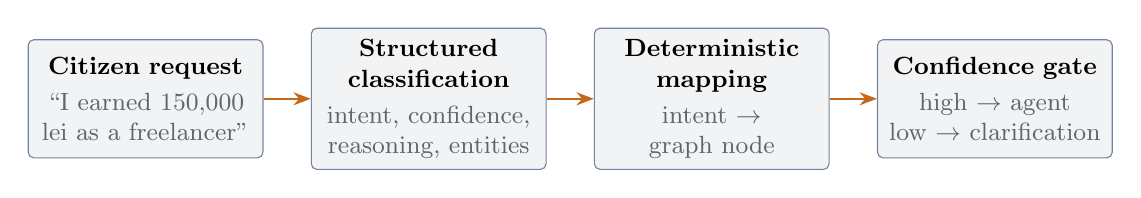
\begin{tikzpicture}[node distance=6mm, every node/.style={font=\small},
      box/.style={draw=navy!60, fill=navy!6, rounded corners=2pt, align=center,
                  inner sep=4pt, text width=27mm, minimum height=15mm},
      ar/.style={-{Stealth[length=2.2mm]}, draw=amber, line width=0.8pt}]
    \node[box] (q) {\textbf{Citizen request}\\[2pt]\aside{``I earned 150,000 lei as a freelancer''}};
    \node[box, right=of q] (c) {\textbf{Structured classification}\\[2pt]\aside{intent, confidence, reasoning, entities}};
    \node[box, right=of c] (m) {\textbf{Deterministic mapping}\\[2pt]\aside{intent $\rightarrow$ graph node}};
    \node[box, right=of m] (g) {\textbf{Confidence gate}\\[2pt]\aside{high $\to$ agent\\low $\to$ clarification}};
    \draw[ar] (q) -- (c); \draw[ar] (c) -- (m); \draw[ar] (m) -- (g);
  \end{tikzpicture}
  \end{center}
  \vfill
  \begin{itemize}
    \item The LLM classifies; it does not decide the route. A fixed table turns the
      predicted intent into a graph node, so the routing step itself stays inspectable.
    \item Below the confidence threshold the request goes to clarification, even when an
      intent was assigned. Dispatching the wrong specialist here means computing the wrong tax.
  \end{itemize}
\end{frame}

\begin{frame}{Five workflows over four shared services}
  \begin{columns}[T]
    \begin{column}{0.5\textwidth}
      \lab{DOMAIN AGENTS}
      \begin{itemize}\small
        \item \textbf{PFA / Freelancer} --- \emph{Declara\c{t}ia Unic\u{a}} (D212); pension
          contribution 25\% above 12 minimum salaries (48,600 RON in 2026), health 10\% above 6
        \item \textbf{Property sale} --- 3\% under three years of ownership, 1\% at or above
        \item \textbf{Rental income} --- contract registration with ANAF, 10\% flat tax
        \item \textbf{Certificate} --- \emph{certificat de atestare fiscal\u{a}}
        \item \textbf{e-Factura} --- B2B and B2C invoicing, XML generation, status monitoring
      \end{itemize}
    \end{column}
    \begin{column}{0.47\textwidth}
      \lab{SHARED SERVICES}
      \begin{itemize}\small
        \item \textbf{Document intake} --- OCR and schema validation; below 80\% confidence
          the document goes to manual review
        \item \textbf{RAG} --- retrieval over indexed sections of the Romanian Tax Code,
          so an explanation can be traced to a source
        \item \textbf{Calculation} --- decimal arithmetic, no floating point; rates read
          from configuration and updated yearly without code changes
        \item \textbf{Payment} --- builds the request, returns a Ghi\c{s}eul.ro redirect URL
      \end{itemize}
    \end{column}
  \end{columns}
  \vfill
  \begin{keypoint}
    Design rule: the model interprets, deterministic code computes.
  \end{keypoint}
\end{frame}

\begin{frame}{Why this substrate}
  A bare orchestration library leaves model access, retrieval, retry logic, escalation and
  document storage to be assembled separately. The UiPath Python SDK supplies them next to
  LangGraph, in one execution environment.
  \vfill
  \begin{columns}[T]
    \begin{column}{0.47\textwidth}
      \begin{itemize}\small
        \item \texttt{UiPathChat} --- model access through the platform gateway (GPT-4o)
        \item \texttt{ContextGroundingRetriever} --- retrieval over indexed knowledge bases
        \item Buckets, queues and human review tasks for storage and escalation
      \end{itemize}
    \end{column}
    \begin{column}{0.47\textwidth}
      \begin{itemize}\small
        \item Government boundaries are \textbf{mocked}, but keep the request and response
          schemas of the real services
        \item In production these become robotic processes; some portals still require
          browser interaction rather than an API
      \end{itemize}
    \end{column}
  \end{columns}
  \vfill
  \begin{sidepoint}
    The mocks are what make a controlled robustness study possible without live access to
    government systems.
  \end{sidepoint}
\end{frame}

%% ========================================================= fault injection ==
\section{Fault injection at the boundaries}

\begin{frame}{The failure mode that matters here}
  \begin{center}
  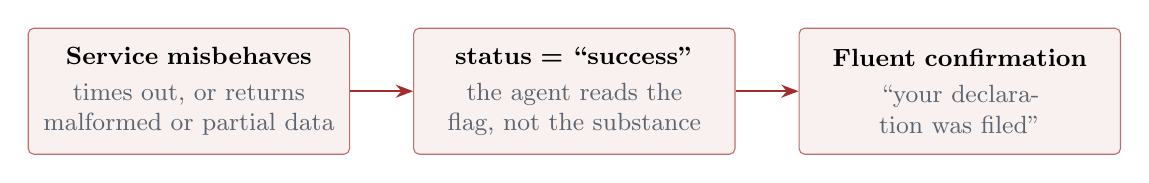
\begin{tikzpicture}[every node/.style={font=\small},
      box/.style={draw=brick!70, fill=brick!7, rounded corners=2pt, align=center,
                  inner sep=4pt, text width=38mm, minimum height=16mm},
      ar/.style={-{Stealth[length=2.2mm]}, draw=brick, line width=0.8pt}]
    \node[box] (a) {\textbf{Service misbehaves}\\[2pt]\aside{times out, or returns malformed or partial data}};
    \node[box, right=8mm of a] (b) {\textbf{status = ``success''}\\[2pt]\aside{the agent reads the flag, not the substance}};
    \node[box, right=8mm of b] (c) {\textbf{Fluent confirmation}\\[2pt]\aside{``your declaration was filed''}};
    \draw[ar] (a) -- (b); \draw[ar] (b) -- (c);
  \end{tikzpicture}
  \end{center}
  \vfill
  An agent that trusts a service-reported success flag and looks no further will build a
  confident answer on top of a broken response. The conversation reads as normal while
  invalid state passes underneath it.
  \vfill
  \begin{keypoint}
    In a regulated setting this is worse than a visible crash: nothing signals that
    anything went wrong.
  \end{keypoint}
\end{frame}

\begin{frame}[plain]
  \centering
  {\color{navy}\large\bfseries The injector: one draw per boundary crossing}\\[1.5mm]
  \includegraphics[width=\textwidth, height=0.95\textheight, keepaspectratio]%
                  {l3pngbigtext.drawio.png}
\end{frame}

\begin{frame}{Four chaos operators}
  \begin{table}
    \small
    \begin{tabular}{@{}llll@{}}
      \toprule
      \textbf{Operator} & \textbf{Effect on the call} & \textbf{Payload} & \textbf{Visible to the agent?}\\
      \midrule
      Timeout    & raises \texttt{TimeoutError}                & none returned & \textcolor{teal}{always}\\
      Delay      & sleeps $\mathcal{U}[1, \Delta t_{\max}]$ ms & unchanged     & \textcolor{brick}{never}\\
      Partial    & one random field set to \texttt{None}       & mutated       & \textcolor{brick}{usually not}\\
      Corruption & one random field set to a sentinel          & mutated       & \textcolor{brick}{usually not}\\
      \bottomrule
    \end{tabular}
  \end{table}
  \vfill
  \begin{itemize}
    \item Three parameters: seed $s$ for deterministic replay, per-call injection rate
      $\eta$, delay bound $\Delta t_{\max}$. At $\eta = 0$ the nominal system is recovered
      unchanged.
    \item 19 instrumented boundary operations: 8 function-level mock tools and 11
      class-method wrappers across three mocked external systems.
    \item Operators are drawn uniformly, so each accounts for a quarter of injected faults.
      The injector is a separate wrapper layer; the nominal service logic is untouched.
  \end{itemize}
\end{frame}

\begin{frame}{Why the faults are silent}
  Agent control flow usually turns on a single field: a predicate such as
  \texttt{status == "success"}. The rest of the response object carries content the branch
  never inspects.
  \vfill
  \begin{center}
  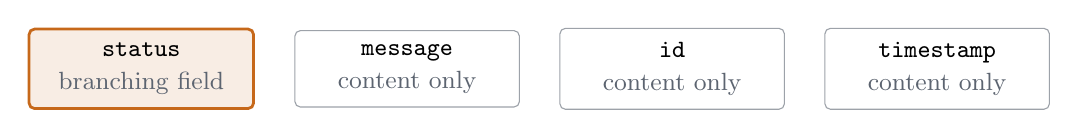
\begin{tikzpicture}[every node/.style={font=\small},
      f/.style={draw=slate!60, fill=white, rounded corners=2pt, align=center,
                inner sep=5pt, text width=25mm},
      gate/.style={draw=amber, fill=amber!12, line width=1pt}]
    \node[f, gate] (s) {\texttt{status}\\[1pt]\aside{branching field}};
    \node[f, right=5mm of s] (m) {\texttt{message}\\[1pt]\aside{content only}};
    \node[f, right=5mm of m] (i) {\texttt{id}\\[1pt]\aside{content only}};
    \node[f, right=5mm of i] (t) {\texttt{timestamp}\\[1pt]\aside{content only}};
  \end{tikzpicture}
  \end{center}
  \vfill
  \begin{columns}[T]
    \begin{column}{0.52\textwidth}
      A single-field perturbation that misses \texttt{status} leaves the predicate true,
      so the agent takes the success branch anyway. For a response with $|\mathcal{F}|$
      fields, one of which gates control flow:
      \[ P(\text{silent}) = 1 - \frac{1}{|\mathcal{F}|} \]
    \end{column}
    \begin{column}{0.44\textwidth}
      \begin{exampleblock}{Expected silent rate}
        \[ \underbrace{0.25}_{\text{delay}} + \underbrace{2 \times 0.25 \times 0.75}_{\text{partial, corruption}} = \mathbf{0.625} \]
        \aside{Timeout, the remaining quarter, always raises.}
      \end{exampleblock}
    \end{column}
  \end{columns}
\end{frame}

%% =============================================================== evaluation ==
\section{Results}

\begin{frame}{Experimental setup}
  \begin{columns}[T]
    \begin{column}{0.47\textwidth}
      \lab{PROTOTYPE}
      \begin{itemize}\footnotesize
        \item Python 3.11, LangGraph 0.2, GPT-4o via the UiPath LLM Gateway
        \item No live network traffic: every government call goes through the mocked
          boundary layer
      \end{itemize}
      \lab{RUNS}
      \begin{itemize}\footnotesize
        \item $N = 100$ boundary calls, each an independent trial with at most one
          injected fault
        \item Sampled across the 8 mock tools, weighted by call frequency in the five
          demo workflows
        \item $\eta \in \{0, 0.25, 0.50, 0.75, 1.00\}$, $s = 17$, $\Delta t_{\max} = 250$\,ms
      \end{itemize}
    \end{column}
    \begin{column}{0.47\textwidth}
      \lab{CLASSIFYING AN OUTCOME}
      \begin{block}{Detectable}
        \footnotesize The response signals failure: an exception propagates, or an explicit
        error or degraded-service notice reaches the user.
      \end{block}
      \begin{alertblock}{Silent pass-through}
        \footnotesize Anything else. The citizen-facing answer looks normal.
      \end{alertblock}
      \aside{The unit of analysis is the call, not the session --- a full workflow
      crosses several boundaries.}
    \end{column}
  \end{columns}
\end{frame}

\begin{frame}{One trace, in full}
  A citizen reports PFA income of 150,000 RON and asks what is owed.
  \vfill
  \begin{columns}[T]
    \begin{column}{0.48\textwidth}
      \small
      \begin{enumerate}
        \item Entry Agent classifies \texttt{pfa\_d212\_filing}, confidence 0.95
        \item PFA Agent computes pension 9,900 RON and health 1,980 RON, total 11,880 RON
        \item On the confirmation turn, the SPV submission call is intercepted at
          $\eta = 1.0$, $s = 17$
      \end{enumerate}
      \medskip
      \begin{sidepoint}
        \scriptsize\ttfamily
        [WARN] fault injected | op=mock\_spv\_submit\_d212 | type=partial
      \end{sidepoint}
    \end{column}
    \begin{column}{0.48\textwidth}
      \small
      The \texttt{message} field of \texttt{SPVSubmissionResult} was set to \texttt{None}.
      \texttt{status} stayed \texttt{"success"}, so the agent followed the success branch
      and answered:
      \medskip
      \begin{keypoint}
        \small\emph{``The D212 declaration was successfully submitted!
        ID: D212-01B66C85C3, Timestamp: 2026-03-27T22:20:32.''}
      \end{keypoint}
      \medskip
      \aside{Four fields, one of them gating. A single-field fault stays invisible with
      probability $0.75$. Nothing about this trace is accidental.}
    \end{column}
  \end{columns}
\end{frame}

\begin{frame}{About 63\%, at every injection rate}
  \begin{table}
    \small
    \begin{tabular}{@{}rrrrrrrr@{}}
      \toprule
      $\eta$ & Faults & TO & DL & PT & CR & Silent & Detectable\\
      \midrule
      0.00 & 0   & 0  & 0  & 0  & 0  & 0 (---) & 0 (---)\\
      0.25 & 25  & 6  & 6  & 7  & 6  & 16 (64\%) & 9 (36\%)\\
      0.50 & 50  & 12 & 13 & 12 & 13 & 32 (64\%) & 18 (36\%)\\
      0.75 & 75  & 19 & 19 & 18 & 19 & 47 (63\%) & 28 (37\%)\\
      1.00 & 100 & 25 & 25 & 25 & 25 & \alert{63 (63\%)} & 37 (37\%)\\
      \bottomrule
    \end{tabular}
    \\[0.3em]
    \aside{$N = 100$ calls, $s = 17$, $\Delta t_{\max} = 250$\,ms.
    TO, DL, PT, CR: timeout, delay, partial, corruption.}
  \end{table}
  \vfill
  \begin{itemize}
    \item The measured rate sits on the predicted 0.625. Raising $\eta$ raises the
      \emph{count} of silent faults, not their proportion.
    \item Delay faults added $125.5 \pm 72.2$\,ms per affected call, matching the mean of
      $\mathcal{U}[1,250]$. At $\eta = 0.50$ that is roughly 65\,ms per scenario.
    \item Because the rate follows from the operator mix and the schema, it can be predicted
      before the system runs --- and lowered by changing what the branch inspects.
  \end{itemize}
\end{frame}

\begin{frame}{Cost is not the obstacle}
  \vfill
  \begin{columns}[T]
    \begin{column}{0.32\textwidth}
      \centering
      \lab{PER SESSION}\\[0.4em]
      {\Huge\bfseries\color{navy}\$0.05}\\[0.5em]
      \aside{one classification, two to three domain turns, one retrieval step}
    \end{column}
    \begin{column}{0.32\textwidth}
      \centering
      \lab{SMALL OFFICE}\\[0.4em]
      {\Huge\bfseries\color{navy}\$51}\\[0.5em]
      \aside{per month, at 50 sessions a day}
    \end{column}
    \begin{column}{0.32\textwidth}
      \centering
      \lab{LARGE AGENCY}\\[0.4em]
      {\Huge\bfseries\color{navy}\$5,060}\\[0.5em]
      \aside{per month, at 5,000 sessions a day}
    \end{column}
  \end{columns}
  \vfill
  \begin{itemize}\small
    \item About 20,000 input and 2,100 output tokens per session, priced at \$1.25 per
      million input and \$10.00 per million output tokens, over 22 working days a month.
      Licensing, infrastructure and maintenance are excluded.
    \item Cost scales linearly and stays modest. Routing with a smaller model, keeping the
      capable one for domain reasoning, pushes it lower.
  \end{itemize}
  \vfill
  \begin{keypoint}
    What stands in the way of deployment is assurance, not arithmetic.
  \end{keypoint}
\end{frame}

%% =============================================================== conclusion ==
\section{Conclusion}

\begin{frame}{Interface coherence is not evidence of correctness}
  \begin{columns}[T]
    \begin{column}{0.47\textwidth}
      \lab{WHAT WE FOUND}
      \begin{itemize}\small
        \item An operational multi-agent architecture covering five Romanian fiscal
          workflows, on LangGraph and the UiPath Python SDK
        \item A silent pass-through rate near 63\%, stable across injection rates and
          matching a closed-form prediction
        \item The cause sits in response schemas and branching predicates, not in
          incidental bugs
        \item Inference cost is modest at institutional volumes
      \end{itemize}
    \end{column}
    \begin{column}{0.47\textwidth}
      \lab{WHAT COMES NEXT}
      \begin{itemize}\small
        \item \textbf{Output contracts} --- check responses against explicit validity
          conditions before they reach the citizen: missing submission identifiers,
          invalid payment codes, incomplete certificate responses
        \item \textbf{Trace-based assurance} --- structured message-action traces,
          deterministic replay, action-level governance
        \item \textbf{Beyond taxation} --- other public-service domains reusing the
          orchestration and shared services layers
      \end{itemize}
    \end{column}
  \end{columns}
  \vfill
  \begin{keypoint}
    A fault that never changes the branch will never announce itself. Validation has to
    happen at the output, where the contract is.
  \end{keypoint}
\end{frame}

\begin{frame}[standout]
  Thank you\\[0.6em]
  {\normalsize\normalfont Radu-Mihai Gheorghe}\\[1.4em]
  {\small\normalfont\ttfamily github.com/radugheo/agentic-public-administration}
\end{frame}

\end{document}
